

\appendix

\section{Cross Modal Contrastive Learning}

Yusuf Aytar, Carl Vondrick, and Antonio Torralba. Sound-
net: Learning sound representations from unlabeled video.
In Adv. Neural Inform. Process. Syst., 2016. 

Andrew Owens, Jiajun Wu, Josh McDermott, William Free-
man, and Antonio Torralba. Ambient sound provides super-
vision for visual learning. In Eur. Conf. Comput. Vis., 2016.

Hang Zhao, Chuang Gan, Andrew Rouditchenko, Carl Von-
drick, Josh McDermott, and Antonio Torralba. The sound of
pixels. In Eur. Conf. Comput. Vis., September 2018.

\section{Modeling video and speech}
Here we sketch some ideas for how to model videos with spoken
narration or dialog, based on related work.

\subsection{Separate encoders}
This is the approach taken in \citet{rouditchenko2020avlnet} where the
video encoder and the audio encoder both separately embed their
respective modality as a vector. The loss function is contrastive,
based on max-margin softmax \citep{ilharco-etal-2019-large}, where the
softmax is applied to pairwise dot products between modality-specific
vectors:

\begin{equation}
  \label{eq:mms}
  L(\mathbf{x}, \mathbf{y}) = - \mean_i \left(
    \log \frac{\exp(\mathbf{x}_i\cdot \mathbf{y}_i-\delta)}
    { \exp(\mathbf{x}_i\cdot \mathbf{y}_i-\delta) + \sum_{j\neq i}
      \exp(\mathbf{x}_i \cdot \mathbf{y}_j)  }
  \right)
\end{equation}
where $\mathbf{x, y}$ are modality-specific vectors and $\delta$ is the
margin. The second term in the denominator sums over the negative
examples.

The advantage of this type of approach is its simplicity and the fact
that there is a single vector representation for the whole speech
fragment.

\subsection{Multiple instance learning}
In the approach introduced in \citet{miech2020end} the objective is
basically \cref{eq:mms} without the margin, and multiple positive
examples: instead of a single positive example as in \cref{eq:mms}, a
set of potentially positive examples is sampled from closely
co-occuring video-text fragments (see \cref{fig:positive}. This is
supposed to address to some extent the issue that the content of the
video and the corresponding speech are only weakly and noisily
synchronized. There is a lot of verbiage about this in the paper, but
it seems like a pretty trivial idea, and I'm not sure why it works
better than simply using longer video-text segments (it does seem to
work better).
\begin{figure}
  \centering
  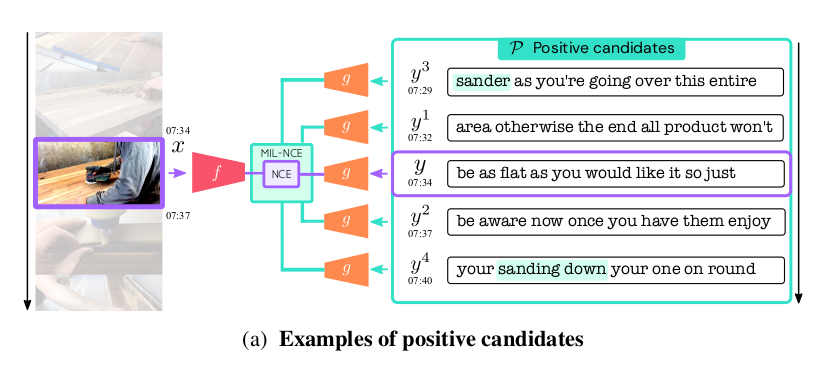
\includegraphics[scale=0.3]{positive}
  \caption{Examples of positive examples from \citet{miech2020end}.}
  \label{fig:positive}
\end{figure}

\subsection{Matchmap}
The matchmap is a concept introduced in \citet{harwath2018jointly} and
which specifies the affinity between each region of the two
dimensional visual feature map and each frame in the associated audio,
i.e.\ it is a three-dimensional tensor. The similarity between the
image and the speech can be computed by a number of scoring functions
which aggregate across these dimensions in different ways: the one
which tended to work best was defined as:
\begin{equation}
  \label{eq:misa}
  \mathrm{MISA}(M) = \mean_t \left(\max_{r,c}(M_{r,c,t})\right)
\end{equation}

The extension of this idea to videos associated with speech would
simply add an extra dimension to the matchmap, corresponding to time
in the visual domain. This would make the matchmap a four-dimensional
tensor, specifying the affinity between each region of the each frame
of the video with a frame of the audio. Overall similarity between
video and speech would involve a scoring function aggregating over
the four dimensions: the equivalent to MISA would be:
\begin{equation}
  \label{eq:misa4}
  \mathrm{MISA}_4(M) = \mean_t \left(\max_{r,c,\tau}(M_{r,c,\tau,t})\right),
\end{equation}
where $t$ is time in the audio modality, and $\tau$ is time in the
video modality. This function has the effect that for each frame of
the audio, it finds the best matching frame/region (let us call this
{\it fragment}) of the video, and averages over the scores of these
matches. It does this without encouraging any sort of structure to
this alignment, for example nothing prevents the same fragment of the
video to be the best match for each frame of the audio.

This approach does, \textit{not per}, se produce a single vector
representing an utterance and thus if audio-audio retrieval or
similarity metric is desired, something more complex than a simple
cosine similarity would be needed:

\begin{itemize}
  \label{itemize:pool}
\item Mean or max pooling of features across frames in order to obtain
  a single vector for the utterance;
\item Dynamic Time Warping if audio-audio similarity metric is needed.
\end{itemize}



\subsection{Transformer-based models}

\subsubsection{Contrastive bi-modal transformer}
\label{sec:cbmt}
The model proposed in \citet{sun2019videobert} uses the BERT
architectire directly to model video-text data. The video is converted
to high-level visual tokens and concatenated with transcribed audio. A
video-text datapoint is transformed to the the sequence
$$(\texttt{[CLS]} w_1\ldots w_n \texttt{[>]} v_1 \dots v_m
\texttt{[SEP]})$$ and used as input to the standard BERT architecture
and trained adapting the BERT training objectives. The \texttt{[CLS]}
token is used as a joint representation of the video-text datapoint. A
similar approach could be used for video-audio data: tokens can
correspond to video and/or audio frame features. For training,
BERT-like objectives could be used; a interesting alternative would be
to adapt this architecture to use with the contrastive loss. We would
represent in input as
$$(\texttt{[AUD]} w_1\ldots w_n \texttt{[VID]} v_1 \dots v_m)$$ using
\texttt{[AUD]} and \texttt{[VID]} as pooled representations of audio
and video respectively, and use these with the loss from \cref{eq:mms}
(or similar), identifying these representations with $x_m$ and $y_n$, respectively
in the formula.


\subsubsection{VilBERT}
The ViLBERT paper \citep{lu2019vilbert} uses a transformer with
so-called co-attention to model data which consist of images
(represented as a collection of regions) and text. There are not many
details in the paper about the actual formulation of these
co-attention heads, but there is a picture: see \cref{fig:coatt}.
\begin{figure}
  \centering
  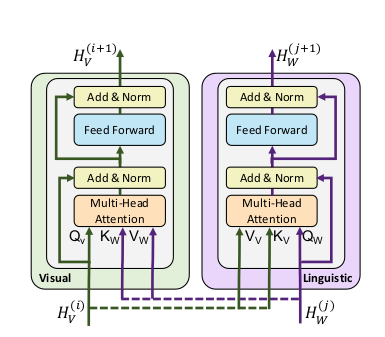
\includegraphics[scale=0.3]{coatt.png}
  \caption{ViLBERT consists of two parallel streams for visual and
    linguistic data that interact through co-attention transformer
    layers (image from \citep{lu2019vilbert}).}
  \label{fig:coatt}
\end{figure}
In principle this architecture could also be suitable for modeling
video-audio data: instead if image regions we'd be using video frames.

\subsubsection{CBT (contrastive bidirectional transformer)}
\citet{sun2019learning} is rather convoluted: there are two BERT-like
encoders, as well as a separate cross-modal transformer, with a
contrastive training objective, which unlike \cref{sec:cbmt} uses a
simple joint representation for both modalities.



